\documentclass{article}
\usepackage[utf8]{inputenc}
\usepackage{listings}
\usepackage{multimedia} % to embed movies in the PDF file
\usepackage{graphicx}
\usepackage{comment}
\usepackage[english]{babel}
\usepackage{amsmath}
\usepackage{amsfonts}
\usepackage{subfigure}
\usepackage{wrapfig}
\usepackage{multirow}
\usepackage{tikz}
\usepackage{verbatim}
%!TEX root = main.tex



\newcommand{\eref}[1]{\mbox{\rm(\ref{#1})}}
\newcommand{\tref}[1]{\mbox{\rm\ref{#1}}}
\newcommand{\set}[2]{\left\{ #1 \; : \; #2 \right\} }
\newcommand{\deq}{\raisebox{0pt}[1ex][0pt]{$\stackrel{\scriptscriptstyle{\rm def}}{{}={}}$}}

\newcommand {\DS} {\displaystyle}

\newcommand{\real}{\mathbb{R}}



\newcommand {\half} {\mbox{$\frac{1}{2}$}}
\newcommand{\force}{{\mathbf{f}}}
\newcommand{\strain}{{\boldsymbol{\varepsilon}}}
\newcommand{\stress}{{\boldsymbol{\sigma}}}
\renewcommand{\div}{{\boldsymbol{\nabla}}}

\newcommand {\cA} {{\cal A}}
\newcommand {\cB} {{\cal B}}
\newcommand {\cC} {{\cal C}}
\newcommand {\cD} {{\cal D}}
\newcommand {\cE} {{\cal E}}
\newcommand {\cK} {{\cal K}}
\newcommand {\cL} {{\cal L}}
\newcommand {\cP} {{\cal P}}
\newcommand {\cQ} {{\cal Q}}
\newcommand {\cR} {{\cal R}}
\newcommand {\cV} {{\cal V}}
\newcommand {\cW} {{\cal W}}
\newcommand {\CC} {{\cal C}}
\newcommand {\CD} {{\cal D}}
\newcommand {\CH} {{\cal H}}
\newcommand {\CS} {{\cal S}}
\newcommand {\CU} {{\cal U}}
\newcommand {\CY} {{\cal Y}}



\newcommand{\bzero}{\mathbf{0}}
\newcommand{\ba}{\mathbf{a}}
\newcommand{\bb}{\mathbf{b}}
\newcommand{\bc}{\mathbf{c}}
\newcommand{\bd}{\mathbf{d}}
\newcommand{\be}{\mathbf{e}}
\newcommand{\bg}{\mathbf{g}}
\newcommand{\bh}{\mathbf{h}}
\newcommand{\bl}{\mathbf{l}}
\newcommand{\bn}{\mathbf{n}}
\newcommand{\bp}{\mathbf{p}}
\newcommand{\bq}{\mathbf{q}}
\newcommand{\br}{\mathbf{r}}
\newcommand{\bs}{\mathbf{s}}
\newcommand{\bt}{\mathbf{t}}
\newcommand{\bu}{\mathbf{u}}
\newcommand{\bv}{\mathbf{v}}
\newcommand{\bw}{\mathbf{w}}
\newcommand{\bx}{\mathbf{x}}
\newcommand{\by}{\mathbf{y}}
\newcommand{\bz}{\mathbf{z}}
\newcommand{\bA}{{\mathbf A}}
\newcommand{\bB}{\mathbf{B}}
\newcommand{\bC}{\mathbf{C}}
\newcommand{\bD}{\mathbf{D}}
\newcommand{\bE}{\mathbf{E}}
\newcommand{\bF}{\mathbf{F}}
\newcommand{\bG}{\mathbf{G}}
\newcommand{\bH}{\mathbf{H}}
\newcommand{\bI}{\mathbf{I}}
\newcommand{\bJ}{\mathbf{J}}
\newcommand{\bK}{\mathbf{K}}
\newcommand{\bL}{\mathbf{L}}
\newcommand{\bM}{\mathbf{M}}
\newcommand{\bN}{\mathbf{N}}
\newcommand{\bO}{\mathbf{O}}
\newcommand{\bP}{\mathbf{P}}
\newcommand{\bQ}{\mathbf{Q}}
\newcommand{\bR}{\mathbf{R}}
\newcommand{\bS}{\mathbf{S}}
\newcommand{\bU}{\mathbf{U}}
\newcommand{\bV}{\mathbf{V}}
\newcommand{\bW}{\mathbf{W}}
\newcommand{\bX}{\mathbf{X}}
\newcommand{\bY}{\mathbf{Y}}
\newcommand{\bZ}{\mathbf{Z}}

\newcommand{\bgamma}{{\boldsymbol{\gamma}}}
\newcommand{\bmu}{{\boldsymbol{\mu}}}
\newcommand{\bkappa}{{\boldsymbol{\kappa}}}
\newcommand{\blambda}{{\boldsymbol{\lambda}}}
\newcommand{\bLambda}{{\boldsymbol{\Lambda}}}
\newcommand{\bpi}{{\boldsymbol{\pi}}}
\newcommand{\bPi}{{\boldsymbol{\Pi}}}
\newcommand{\btheta}{{\boldsymbol{\theta}}}
\newcommand{\bTheta}{{\boldsymbol{\Theta}}}
\newcommand{\bSigma}{{\boldsymbol{\Sigma}}}





\title{AMATH 570 Assignment 4}
\author{Cade Ballew}
\date{November 24, 2021}

\begin{document}

\maketitle

\section{Problem 1 (15.4)}
Using chebfun to investigate the Lebesgue constant for the set of $n$ Chebyshev points with the endpoints removed, we get what appears to be a linear $O(n)$ relationship.\\
\includegraphics[]{15-4.eps}\\
See problem15\_4.m for the code that does this. 
\section{Problem 2} 
For completeness, the bound (15.5) is 
\[
||f-p||\leq(\Lambda+1)||f-p^{*}||
\]
where $f$ is the function we are approximating, $\Lambda$ is the Lebesgue constant for a set of interpolation points, $p\in\mathcal{P}_n$ is the interpolant of $f$ at those points, and $p^*\in\mathcal{P}_n$ is the best polynomial approximation.
\subsection{Part a}
Consider the function $f(x)=1/(1+25x^2)$. Using chebfun, we plot both the bound and the true error for both Chebyshev and equispaced points and obtain the following:\\
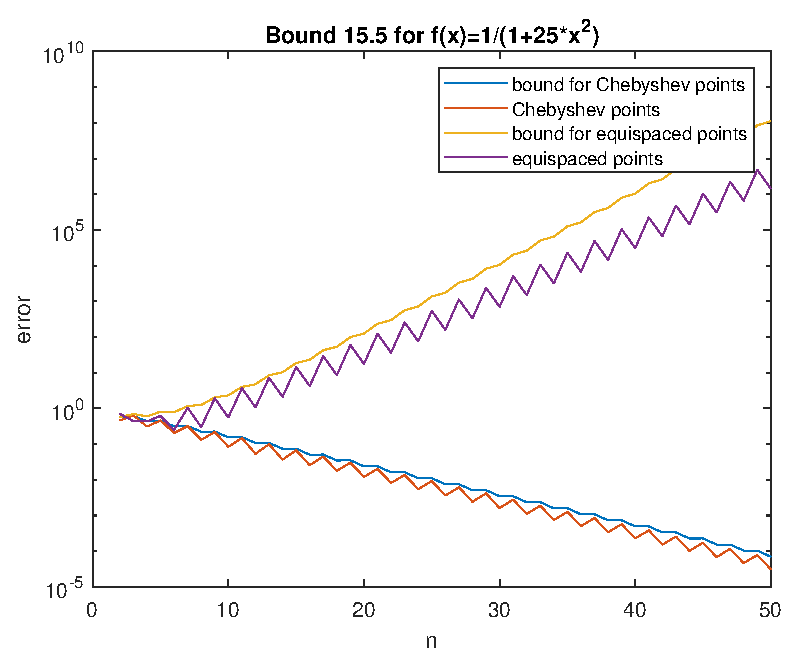
\includegraphics[]{2a.eps}

\subsection{Part b}
Now, consider $f(x)=1/(1+500x^2)$. We again plot both the bound and the true error for both Chebyshev and equispaced points using chebfun and obtain the following: \\
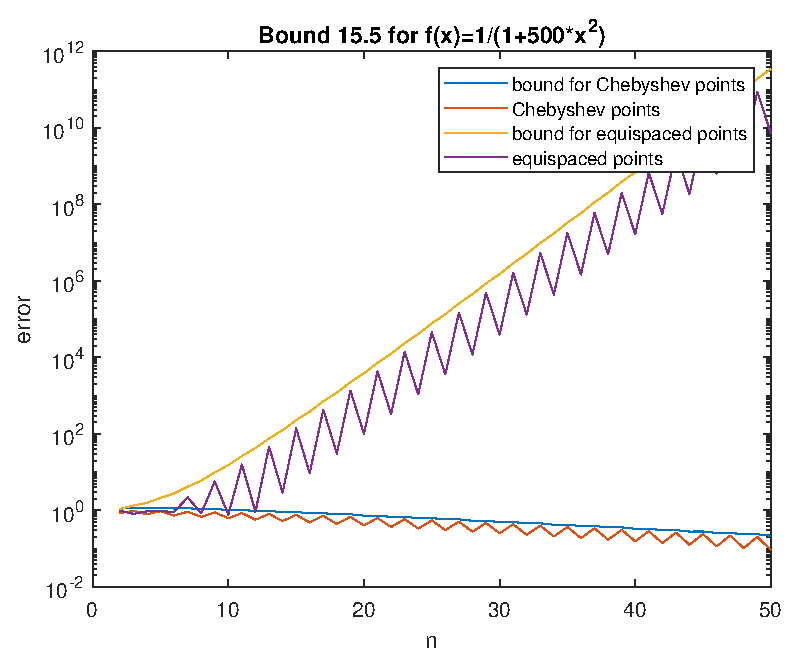
\includegraphics[]{2b.eps}\\
See problem2.m for the relevant MATLAB code.  

\section{Problem 3}
\subsection{Exercise 17.3}
\subsubsection{Part a}
Using chebfun, we construct a quasimatrix $A$ with columns corresponding to $1,x,\ldots,x^5$ on $[-1,1]$. Using the command qr to find an orthonomal set of functions and plotting them, we get \\
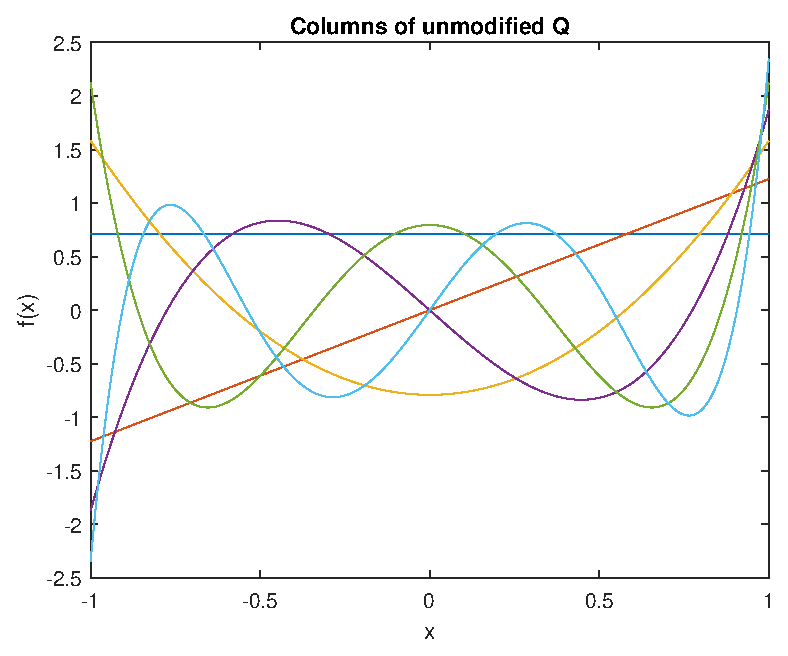
\includegraphics[scale=0.6]{17_1.eps}\\
which appears identical to the following plot of the first 6 Legendre polynomials normalized according to (17.3) which follows.\\
\includegraphics[scale=0.6]{17_2.eps}\\
Indeed, if we plot the absolute value of the difference between the two, we observe\\
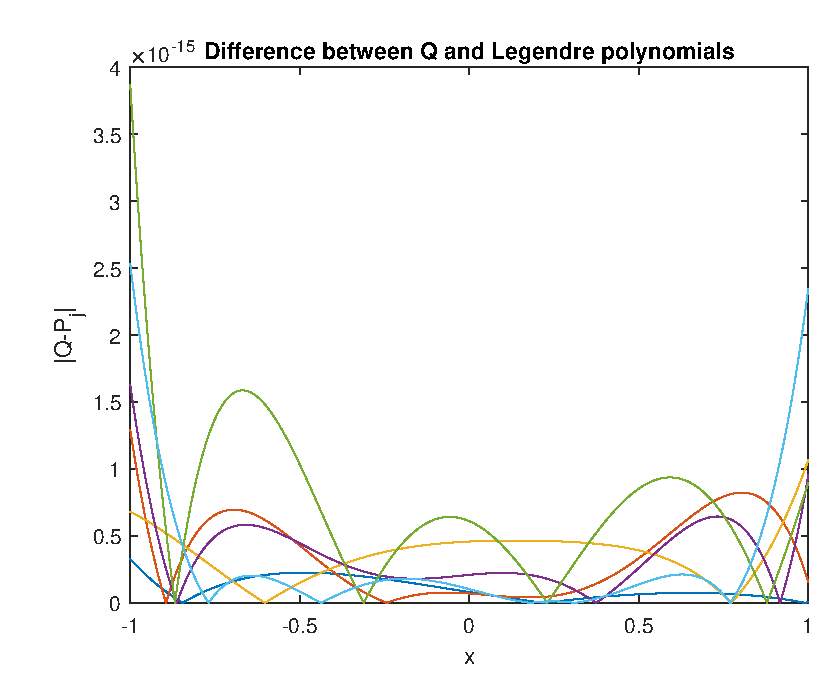
\includegraphics[scale=0.6]{17_3.eps}\\
meaning that they are identical on the order of machine precision. 
\subsubsection{Part b}
Now, we normalize the columns of $Q$ such that they take value 1 at $x=1$ and adjust the rows of $R$ accordingly. To confirm that our modified $Q$ and $R$ still multiply to $A$, we plot the absolute value of the difference between $A$ and $Q*R$\\
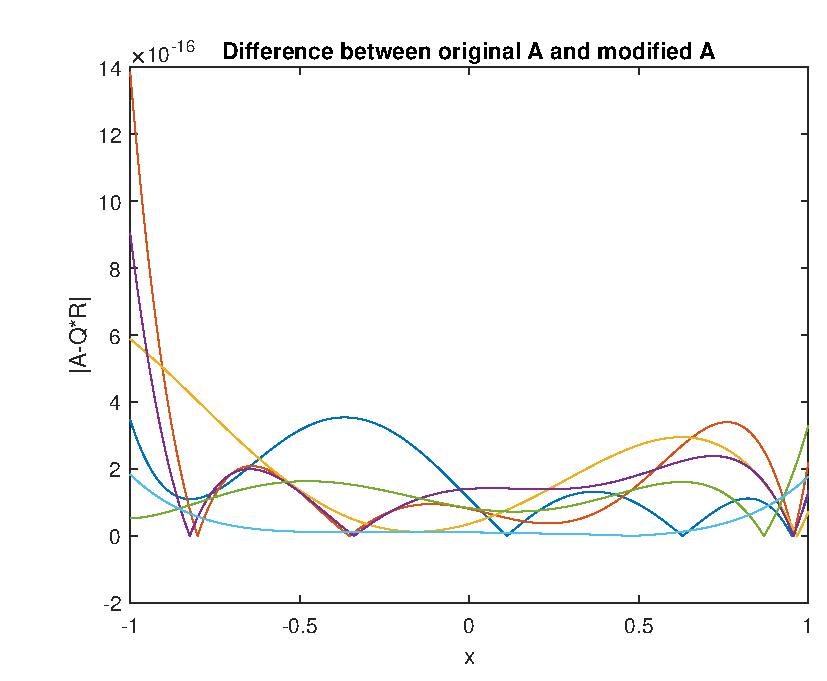
\includegraphics[scale=0.6]{17_4.eps}\\
which shows that they are identical to machine precision. \\
Plotting we columns of the new quasimatrix $Q$, we observe\\
\includegraphics[scale=0.6]{17_5.eps}\\
which now looks identical to the first 6 Legendre polynomials normalized in the same manner. \\
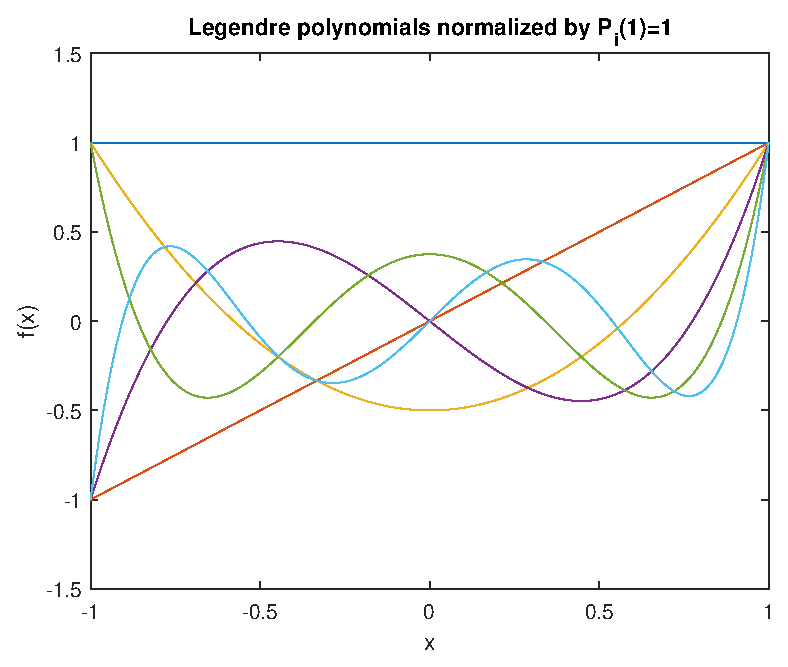
\includegraphics[scale=0.6]{17_6.eps}\\
To confirm this, we again plot the absolute value of their difference which again shows that they are identical to machine precision. \\
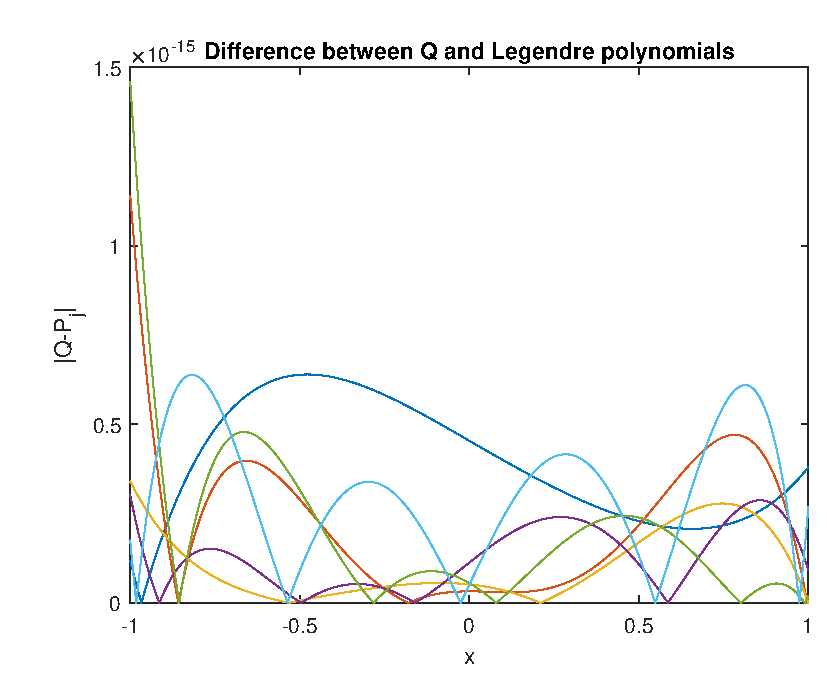
\includegraphics[scale=0.6]{17_7.eps}\\
See problem17\_8.m for the code that produces the plots in this problem.

\subsection{Exercise 17.8}
Let $\{p_n\}$ be the family of monic polynomials associated with the inner product defined in (17.1) and let $q$ be any monic polynomial of degree n. Then, we can write $q$ as 
\[
q(x)=\sum_{k=0}^{n-1}c_kp_k(x)+p_n(x) 
\]
where the coefficient on $p_n$ is 1, because both it and $q$ are monic. We can now write
\begin{align*}
(q,q)&=\int_{-1}^1w(x)\overline{q(x)}q(x)dx\\&=\int_{-1}^1w(x)\left(\overline{\sum_{k=0}^{n-1}c_kp_k(x)+p_n(x)}\right)\left(\sum_{k=0}^{n-1}c_kp_k(x)+p_n(x)\right)dx\\&=
\int_{-1}^1w(x)\left(\sum_{k=0}^{n-1}\overline{c_k}\overline{p_k(x)}+\overline{p_n(x)}\right)\left(\sum_{k=0}^{n-1}c_kp_k(x)+p_n(x)\right)dx.
\end{align*}
Now, the orthogonality of the family $\{p_n\}$ means that $\int_{-1}^1w(x)\overline{p_i(x)}p_j(x)dx=0$ for $i\neq j$, so when we multiply this out and utilize the linearity of the integration operator, the cross-terms will be zero, meaning that 
\begin{align*}
(q,q)&=\sum_{k=0}^{n-1}\int_{-1}^1w(x)\overline{c_k}c_k\overline{p_k(x)}p_k(x)dx+\int_{-1}^1w(x)\overline{p_n(x)}p_n(x)dx\\&=
\sum_{k=0}^{n-1}\overline{c_k}c_k(p_k,p_k)+(p_n,p_n)=\sum_{k=0}^{n-1}|c_k|(p_k,p_k)+(p_n,p_n)\geq(p_n,p_n),
\end{align*}
because $|c_k|,(p_k,p_k)\geq0$ for any $k$.

\section{Problem 4 (18.4)}
\subsection{Part a}
To derive a comrade matrix for the Legendre polynomials in the manner of theorem 18.1, we wish to find a matrix whose eigenvalues are the roots of the polynomial $p(x)=\sum_{k=0}^na_kP_k(x)$. We do this in the same manner as with the Chebyshev polynomials. For the interior, we use the recursive relationship $(k+1)P_{k+1}(x)-kP_{k-1}(x)$ to get that our matrix should map $P_k(x)$ to $xP_k(x)=\frac{k}{2k+1}P_{k-1}(x)+\frac{k+1}{2k+1}P_{k+1}(x)$. For the first row, our matrix should map $P_0(x)$ to $xP_0(x)=P_1(x)$. For the last row, we have the same relationship as with the Chebyshev polynomials but adjusted for our new interior coefficients. Namely,
\[
P_{n-1}(x)\mapsto xP_{n-1}(x)-\frac{n-1+1}{a_n(2(n-1)+1)}(a_0P_0(x)+\ldots+a_nP_n(x)).
\]
Thus, we can write
\[ 
C =
\begin{pmatrix}
0 & 1   \\
1/3 & 0 & 2/3 \\
 & 2/5 & 0 & 3/5 \\
  & & \ddots & \ddots & \ddots \\
  & & & \frac{n-2}{2n-3} & 0 & \frac{n-1}{2n-3} \\
  & & & & \frac{n-1}{2n-1} & 0
\end{pmatrix}
-\frac{n}{a_n(2n-1)}
\begin{pmatrix}
\\
\\
\\
\\
\\
a_0 & a_1 & a_2 & \dots & a_{n-1}
\end{pmatrix}.
\]
Note that the $k$th Legendre polynomial corresponds to the $(k+1)$st row of $C$, so we need to shift the relations above accordingly to explicitly write what $C_{i,j}$ is (see part b for code that does this or problem 5 for it written out explicitly). \\
Then, our theorem is as follows: \\
The roots of the polynomial 
\[
p(x)=\sum_{k=0}^na_kP_k(x), \quad a_n\neq0,
\]
are the eigenvalues of the matrix $C$ as defined above.
\subsection{Part b}
To verify that the comrade matrix for $p=P_0+\ldots+P_5$ has the same eigenvalues are $p$ does roots, we note that $a_i=1$ for $i=0,\ldots,5$ and use MATLAB to construct $C$ for this case which outputs
\begin{verbatim}
The eigenvalues of the comrade matrix are
 -1.000000000000000 + 0.000000000000000i
  0.634846841685047 + 0.225134736423368i
  0.634846841685047 - 0.225134736423368i
 -0.412624619462826 + 0.273188868980396i
 -0.412624619462826 - 0.273188868980396i
\end{verbatim}
and 
\begin{verbatim}
The roots of our polynomial are
 -0.412624619462826 - 0.273188868980397i
 -0.412624619462826 + 0.273188868980397i
  0.634846841685048 - 0.225134736423369i
  0.634846841685048 + 0.225134736423369i
 -1.000000000000001 + 0.000000000000000i
\end{verbatim}
which are given in different order, but match to machine precision as one would expect. \\
See problem18\_4.m for the code that does this.

\section{Problem 5 (19.7)}
\subsection{Part a}
Knowing that the nodes $\{x_j\}$ of the $(n+1)$-point Gauss quadrature are the zeroes of the Legendre polynomial $P_{n+1}$, we wish to find a comrade matrix for which these are its eigenvalues. However, in problem 4, we derived such a comrade matrix for linear combinations of Legendre polynomials. Now, we need an $(n+1)$ by $(n+1)$ matrix, but we have that $a_0=\ldots=a_n=0$ and $a_{n+1}=1$, so the second matrix is the zero matrix and 
\[
A=\begin{pmatrix}
0 & 1   \\
1/3 & 0 & 2/3 \\
 & 2/5 & 0 & 3/5 \\
  & & \ddots & \ddots & \ddots \\
  & & & \frac{n-1}{2n-1} & 0 & \frac{n}{2n-1} \\
  & & & & \frac{n}{2n+1} & 0
\end{pmatrix}
\]
We can reindex our formula from problem 4 to explicitly find the entries of this matrix. Namely, for $k\in\{1,\ldots,n\}$,
\[
\begin{cases}
A_{k,k+1}=\frac{k}{2k-1},\\
A_{k,k-1}=\frac{k-1}{2k-1},\\
A_{k,j}=0, \quad \text{otherwise}.
\end{cases}
\]
Additionally, we have that $A_{1,2}=1$, $A_{n,n+1}=\frac{n}{2n+1}$ and 0 in all other entries. 

\subsection{Part b}
To find a diagonal matrix $D=\text{diag}(d_0,\ldots,d_n)$ such that $B=DAD^{-1}$ is real symmetric, we consider that for $k>1$, 
\[
B_{k,k+1} = d_{k-1}A_{k,k+1}/d_k
\]
and for $k<n+1$
\[
B_{k+1,k} = d_{k}A_{k+1,k}/d_{k-1}.
\]
Because we need $B$ to be symmetric, we can equate these in the interior $2\leq k\leq n$. Thus, 
\[
\frac{d_{k-1}}{d_k}\frac{k}{2k-1}=\frac{d_{k}}{d_{k-1}}\frac{k}{2k+1}.
\]
This yields a quadratic equation 
\[
\frac{d_{k}}{d_{k-1}}=\frac{2k+1}{2k-1}
\]
for which we can consider only the positive solution, because we require that $d_j>0$ for $j\geq1$. Thus,
\[
d_k=d_{k-1}\sqrt{\frac{2k+1}{2k-1}}
\]
for $2\leq k\leq n$. Since we require that $d_0=1$, this recursion actually cancels due to the fact that $2k-1=2(k-1)+1$ and simply yields that $d_k=\sqrt{2k+1}$. Now, using our work above, we find that $B$ has entries 
\[
B_{k,k+1}=\frac{k}{2k-1}\sqrt{\frac{2k-1}{2k+1}}=\frac{k}{\sqrt{(2k-1)(2k+1)}}
\]
and of course, $B_{k+1,k}=B_{k,k+1}$ due to symmetry. More explicitly we can reindex to find that 
\[
B_{k,k-1}=\frac{k-1}{\sqrt{(2k-3)(2k-1)}}.
\]
Of course, the first equation hold for $k=1,\ldots,n$, the second holds for $k=2,\ldots,n+1$, and all other entries are zero. 
\end{document}
